\documentclass[a4paper, 12pt]{report}

\usepackage[dvipsnames]{xcolor}

%%%%%%%%%%%%%%%%
% Set Variables %
%%%%%%%%%%%%%%%%

\def\useItalian{0}  % 1 = Italian, 0 = English

\def\courseName{Advanced Algorithms}

\def\coursePrerequisites{\begin{itemize} \item Progettazione degli Algoritmi \end{itemize}}

\def\book{TODO}

% \def\authorName{Simone Bianco}
% \def\email{bianco.simone@outlook.it}
% \def\github{https://github.com/Exyss/university-notes}
% \def\linkedin{https://www.linkedin.com/in/simone-bianco}

\def\authorName{Alessio Bandiera}
\def\email{alessio.bandiera02@gmail.com}
\def\github{https://github.com/aflaag-notes}
\def\linkedin{https://www.linkedin.com/in/alessio-bandiera-a53767223}

%%%%%%%%%%%%
% Packages %
%%%%%%%%%%%%

\usepackage{../../packages/Nyx/nyx-packages}
\usepackage{../../packages/Nyx/nyx-styles}
\usepackage{../../packages/Nyx/nyx-frames}
\usepackage{../../packages/Nyx/nyx-macros}
\usepackage{../../packages/Nyx/nyx-title}
\usepackage{../../packages/Nyx/nyx-intro}

%%%%%%%%%%%%%%
% Title-page %
%%%%%%%%%%%%%%

\logo{../../packages/Nyx/logo.png}

\if\useItalian1
    \institute{\curlyquotes{\hspace{0.25mm}Sapienza} Università di Roma}
    \faculty{Ingegneria dell'Informazione,\\Informatica e Statistica}
    \department{Dipartimento di Informatica}
    \ifdefined\book
        \subtitle{Appunti integrati con il libro \book}
    \fi
    \author{\textit{Autore}\\\authorName}
\else
    \institute{\curlyquotes{\hspace{0.25mm}Sapienza} University of Rome}
    \faculty{Faculty of Information Engineering,\\Informatics and Statistics}
    \department{Department of Computer Science}
    \ifdefined\book
        \subtitle{Lecture notes integrated with the book \book}
    \fi
    \author{\textit{Author}\\\authorName}
\fi


\title{\courseName}
\date{\today}

% \supervisor{Linus \textsc{Torvalds}}
% \context{Well, I was bored\ldots}

\addbibresource{./references.bib}

%%%%%%%%%%%%
% Document %
%%%%%%%%%%%%

\begin{document}
    \maketitle

    % The following style changes are valid only inside this scope 
    {
        \hypersetup{allcolors=black}
        \fancypagestyle{plain}{%
        \fancyhead{}        % clear all header fields
        \fancyfoot{}        % clear all header fields
        \fancyfoot[C]{\thepage}
        \renewcommand{\headrulewidth}{0pt}
        \renewcommand{\footrulewidth}{0pt}}

        \romantableofcontents
    }

    \introduction

    %%%%%%%%%%%%%%%%%%%%%

    \chapter{TODO}

    \section{TODO}

    \subsection{The Max Cut problem}

    The first problem that will be discussed is the \href{https://en.wikipedia.org/wiki/Maximum_cut}{Maximum Cut} problem (or \tit{Max Cut}, for short). The \tbf{Max Cut problem} --- in the unweighted case --- is a classic combinatorial optimization problem in the branch of \href{https://en.wikipedia.org/wiki/Graph_theory}{graph theory}, in which we seek to partition the vertices of an undirected graph into two disjoint subsets while maximizing the number of edges that have endpoints in both subsets. More formally, we will define a \tbf{cut} of a graph as follows.

    \begin{frameddefn}{Cut}
        Given an undirected graph $G = (V, E)$, and a subset of its vertices $S \subseteq V$, the \tbf{cut} induced by $S$ on $G$ is defined as follows $$\mathrm{cut}(S) := \{e \in E \quad \abs{S \cap e} = 1\}$$
    \end{frameddefn}

    Note that in the definition above we are defining the cut of a graph through the intersection between a set of vertices $S$ and edges in $E$; this is because, in the undirected case, we will consider the edges of a graph $G = (V, E)$ as sets of 2 elements $$E = \{\{u, v\} \quad u, v \in V\}$$ Therefore, given a set of vertices $S$, the cut induced by $S$ is simply the set of edges that have only one endpoint in $S$ (implying that the other one will be in $V - S$).

    \begin{figure}[H]
        \centering
        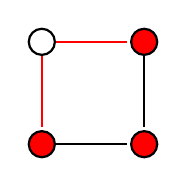
\begin{tikzpicture}[-,>=stealth,shorten >=1pt,auto,node distance=1.3cm, thick,main node/.style={scale=0.9,circle,draw,font=\sffamily\normalsize}]

            \node[circle, draw]  (1) []{};
            \node[circle, draw, fill=red]  (2) [below of = 1]{};
            \node[circle, draw, fill=red]  (3) [right of = 1]{};
            \node[circle, draw, fill=red]  (4) [below of = 3]{};

            % \path[every node/.style={font=\sffamily\small}]

            \draw[-] (1) [red] to (2);
            \draw[-] (1) [red] to (3);
            \draw[-] (2) to (4);
            \draw[-] (3) to (4);

            ;
        \end{tikzpicture}
        \caption{Given the set of red vertices $S$, the green edges represent $\mathrm{cut}(S)$.}
    \end{figure}

    With this definition, we can introduce the \tbf{Max Cut} problem, which is defined as follows.

    \begin{frameddefn}{Max Cut problem}
        Given an undirected graph $G = (V, E)$, determine the set $S \subseteq V$ that maximizes $\abs{\mathrm{cut}(S)}$.
    \end{frameddefn}

    Although this problem is known to be \textsf{APX-Hard} \cite{maxcut}, approximation algorithms and heuristic methods like greedy algorithms and local search are commonly used to find near-optimal solutions.

    For now, we present the following \tbf{randomized algorithm}, which provides a straightforward $\frac{1}{2}$-approximation for the Max Cut problem. This algorithm runs in polynomial time and achieves the approximation guarantee with high probability.

    \begin{framedalgo}{Random Cut}
        Given an undirected graph $G = (V, E)$, the algorithm returns a cut of $G$. \\
        \hrule

        \quad
        \begin{algorithmic}[1]
            \Function{RandomCut}{$G$}
                \State $S := \varnothing$
                \For{$v \in V$}
                    \State Let $c_v$ be the outcome of the flip of an independent fair coin
                    \If{$c_v == \mathrm{heads}$}
                        \State $S = S \cup \{v\}$
                    \EndIf
                \EndFor
                \State \textbf{return} $S$
            \EndFunction
        \end{algorithmic}
    \end{framedalgo}

    Note that this algorithm is powerful, because \tit{it does not care about the structure of the graph in input}, since the output is completely determined by the coin flips performed in the \texttt{for} loop. Now we will prove that this algorithm provides a correct \tbf{expected $\frac{1}{2}$-approximation} of the Max Cut problem.
    
    \begin{framedthm}[label={expected random cut}]{Expected approximation ratio of \textsc{RandomCut}}
        Let $G= (V, E)$ be a graph, and let $S^*$ be an optimal solution to the Max Cut problem on $G$. Then, given $S = \textsc{RandomCut}(G)$, it holds that $$\mathbb E [\abs{\mathrm{cut}(S)}] \ge \dfrac{\abs{\mathrm{cut}(S^*)}}{2}$$
    \end{framedthm}

    \begin{proof}
        By definition, note that $$\forall e \in E \quad e \in \mathrm{cut}(S) \iff \abs{S \cap e} = 1$$ Consider an edge $e = \{v, w\} \in E$; then, by definition $$\{v, w\} \in \mathrm{cut}(S) \iff (v \in S \land w \notin S) \lor (v \notin S \land w \in S)$$ and let $\xi_1$ and $\xi_2$ be these last two events respectively. Then $$\Pr[\xi_1] = \Pr[c_v = \mathrm{heads} \land c_w = \mathrm{tails}]$$ by definition of the algorithm, and by independence of the flips of the fair coins we have that $$\Pr[\xi_1] = \Pr[c_v = \mathrm{heads}] \cdot \Pr[c_w = \mathrm{tails}] = \dfrac{1}{2} \cdot \dfrac{1}{2} = \dfrac{1}{4}$$ Analogously, we can show that $$\Pr[\xi_2] = \dfrac{1}{4}$$ This implies that $$\Pr[e \in \mathrm{cut}(S)] = \Pr[\xi_1 \lor \xi_2] = \Pr[\xi_1] + \Pr[\xi_2] - \Pr[\xi_1 \land \xi_2] = \dfrac{1}{4} + \dfrac{1}{4} - 0 = \dfrac{1}{2}$$ Hence, we have that $$\mathbb E [\abs{\mathrm{cut}(S)}] = \sum_{e \in E}{1 \cdot \Pr[e \in \mathrm{cut}(S)]} = \dfrac{\abs E}{2} \ge \dfrac{\abs{\mathrm{cut}(S^*)}}{2}$$ where the last inequality directly follows from the definition of cut of a graph.
    \end{proof}

    As previously mentioned, this algorithm has an \tbf{expected approximation ratio} of $\frac{1}{2}$, which implies that it may return very bad solutions in some cases, depending on the outcomes of the coin flips. However, thanks to the following algorithm, we can actually transform the \tbf{guarantee of expectations} into a \tbf{guarantee of high probability} --- note that it is possible to show that the previous algorithm provides guarantee of high probability as well, but the proof is much more complex.

    \begin{framedalgo}{$t$-times Random Cut}
        Given an undirected graph $G = (V, E)$ and an integer $t > 0$, the algorithm returns a cut of $G$. \\
        \hrule

        \quad
        \begin{algorithmic}[1]
            \Function{$t$-timesRandomCut}{$G$, $t$}
                \For{$i \in [t]$}
                    \State $S_i := \textsc{RandomCut}(G)$
                \EndFor
                \State \textbf{return} $S \in \argmax_{i \in [t]}{\abs{\mathrm{cut}(S_i)}}$
            \EndFunction
        \end{algorithmic}
    \end{framedalgo}

    The algorithm above simply runs the \textsc{RandomCut} algorithm $t$ times, and returns the set $S_i$ that maximizes the cut, among all the various $S_1, \ldots, S_t$. The following theorem will show that a \tit{reasonable number} of runs of the \textsc{RandomCut} algorithm suffices in order to almost certainly obtain a $\approx \frac{1}{2}$-approximation of any optimal solution.

    \begin{framedthm}{}
        Let $G= (V, E)$ be a graph, and let $S^*$ be an optimal solution to the Max Cut problem on $G$. Then, given $S = \textsc{$t$-timesRandomCut}(G, t)$, it holds that $$\Pr \sbk{\abs{\mathrm{cut}(S)} > \dfrac{1 - \varepsilon}{2} \abs{\mathrm{cut}(S^*)}} > 1 - \delta$$ where $t = \frac{2}{\varepsilon} \ln {\frac{1}{\delta}}$ and $0 < \varepsilon, \delta < 1$.
    \end{framedthm}
    
    \begin{proof}
        For each $i \in [t]$, let $C_i := \abs{\mathrm{cut}(S_i)}$ for each $S_i$ defined by the algorithm, and let $N_i := \abs E - C_i$. Let $0 < \varepsilon < 1$; since $N_i$ is a non-negative random variable, by \href{https://en.wikipedia.org/wiki/Markov%27s_inequality}{Markov's inequality} we have that $$\Pr[N_i \ge (1 + \varepsilon) \mathbb E [N_i]] \le \dfrac{1}{1 + \varepsilon} = 1 - \dfrac{\varepsilon}{1 + \varepsilon} \le 1 - \dfrac{\varepsilon}{2}$$ In particular, this inequality can be rewritten as follows:
        \begin{equation*}
            \begin{split}
                1 - \dfrac{\varepsilon}{2} &\ge \Pr[N_i \ge (1 + \varepsilon) \mathbb E [N_i]] \\
                                           &= \Pr[\abs E - C_i \ge (1 + \varepsilon)(\abs E - \mathbb E [C_i])] \\
                                           &= \Pr[- \varepsilon \abs E \ge C_i - (1 + \varepsilon) \mathbb E [C_i]]
            \end{split}
        \end{equation*}
        As shown in the proof of \cref{expected random cut}, we know that $\mathbb E [C_i] = \frac{\abs E}{2}$, therefore
        \begin{equation*}
            \begin{split}
                1 - \dfrac{\varepsilon}{2} &\ge \Pr[- \varepsilon \abs E \ge C_i - (1 + \varepsilon) \mathbb E [C_i]] \\
                                           &= \Pr \sbk{- \varepsilon \abs E \ge C_i - \dfrac{1 + \varepsilon}{2} \abs E} \\
                                           &= \Pr \sbk{- \varepsilon \dfrac{\abs E}{2} \ge C_i - \dfrac{\abs E}{2}} \\
                                           &= \Pr \sbk{\dfrac{1 - \varepsilon}{2} \abs E\ge C_i} \\
                                           &= \Pr \sbk{(1 - \varepsilon) \mathbb E[C_i] \ge C_i} \\
            \end{split}
        \end{equation*}
        Note that the event in the last probability, namely $$\abs{\mathrm{cut}(S_i)}  \le (1 - \varepsilon) \mathbb E [\abs{\mathrm{cut}(S_i)}]$$ corresponds to a \curlyquotes{bad} solution, i.e. one whose cardinality is at most $(1 - \varepsilon)$-th of the expected value.

        By definition of the algorithm, each of the $t$ runs of the \textsc{RandomCut} algorithm is independent from the others, therefore the probability of \tit{all} the solutions $S_1, \ldots, S_t$ being \curlyquotes{bad} is bounded by $$\Pr[\forall i \in [t]  \quad C_i \le (1 - \varepsilon) \mathbb E [C_i]] = \prod_{i = 1}^t{\Pr[C_i \le (1 - \varepsilon)\mathbb E[C_i]]} \le \rbk{1 - \dfrac{\varepsilon}{2}}^t$$

        Using the fact that $$\forall x \in \R \quad 1 - x \le e^{-x} \implies 1 - \frac{\varepsilon}{2} \le e^{- \frac{\varepsilon}{2}}$$ we have that $$\Pr[\forall i \in [t] \quad C_i \le (1 - \varepsilon) \mathbb E[C_i]] \le \rbk{1 - \dfrac{\varepsilon}{2}}^t \le e^{- \frac{\varepsilon}{2} \cdot t} = e^{- \ln {\frac{1}{\delta}}} = \delta$$

        Therefore, the probability that at least one among $S_1, \ldots, S_t$ is a \curlyquotes{good} solution is bounded by $$\Pr[\exists i \in [t] \quad C_i > (1 - \varepsilon) \mathbb E [C_i]] = 1 - \Pr[\forall i \in [t] \quad C_i \le (1 - \varepsilon) \mathbb E [C_i]] \ge 1 - \delta$$

        placeholder \todo{last part}
    \end{proof}

    Note that this result is \tit{very powerful}: for instance, if $\varepsilon = \delta = 0.1$, we get that $$\Pr[\abs{\mathrm{cut}(S)} > 0.45 \cdot \abs{\mathrm{cut}(S^*)}] \ge 0.9$$ and $t \approx 46$, meaning that we just need to run the \textsc{RandomCut} algorithm approximately 46 times in order to get a solution that is better than a $0.45$-approximation with $90\%$ probability.

    \subsection{The Vertex Cover problem}

    Another very important problem in graph theory is the \href{https://en.wikipedia.org/wiki/Vertex_cover}{Vertex Cover}, which concerns the combinatorial structure of the \tbf{vertex cover}, defined as follows.

    \begin{frameddefn}{Vertex cover}
        Given an undirected graph $G = (V, E)$, a \tbf{vertex cover} of $G$ is a set of vertices $S \subseteq V$ such that $$\forall e \in E \quad \exists v \in S \quad v \in e$$
    \end{frameddefn}

    \begin{figure}[H]
        \centering
        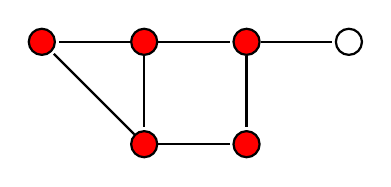
\begin{tikzpicture}[-,>=stealth,shorten >=1pt,auto,node distance=1.3cm, thick,main node/.style={scale=0.9,circle,draw,font=\sffamily\normalsize}]

            \node[circle, draw, fill=red] (1) []{};
            \node[circle, draw, fill=red] (2) [right of = 1]{};
            \node[circle, draw, fill=red] (3) [below of = 1]{};
            \node[circle, draw, fill=red] (4) [below of = 2]{};
            \node[circle, draw, fill=red] (5) [left of = 1]{};
            \node[circle, draw, ] (6) [right of = 2]{};

            \draw[-] (1) to (2);
            \draw[-] (1) to (3);
            \draw[-] (2) to (4);
            \draw[-] (1) to (5);
            \draw[-] (3) to (4);
            \draw[-] (3) to (5);
            \draw[-] (2) to (6);

            ;
        \end{tikzpicture}
        \caption{An example of a vertex cover.}
    \end{figure}

    As shown in figure, a vertex cover is simply a set of vertices that must \tit{cover} all the edges of the graph. Clearly, the trivial vertex cover is representd by $S = V$, but a more interesting solution to the problem is represented by the \tbf{minimum vertex cover}.

    \begin{frameddefn}{Vertex Cover problem}
        The decisional version of the \tbf{Vertex Cover} (VC) is defined as follows: given an undirected graph $G = (V, E)$, determine the vertex cover $S \subseteq V$ of smallest cardinality.
    \end{frameddefn}

    \begin{figure}[H]
        \centering
        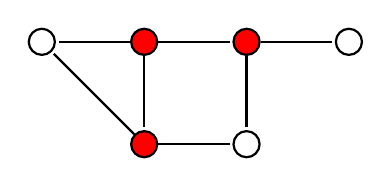
\begin{tikzpicture}[-,>=stealth,shorten >=1pt,auto,node distance=1.3cm, thick,main node/.style={scale=0.9,circle,draw,font=\sffamily\normalsize}]

            \node[circle, draw, fill=red] (1) []{};
            \node[circle, draw, fill=red] (2) [right of = 1]{};
            \node[circle, draw, fill=red] (3) [below of = 1]{};
            \node[circle, draw, ] (4) [below of = 2]{};
            \node[circle, draw, ] (5) [left of = 1]{};
            \node[circle, draw, ] (6) [right of = 2]{};

            \draw[-] (1) to (2);
            \draw[-] (1) to (3);
            \draw[-] (2) to (4);
            \draw[-] (1) to (5);
            \draw[-] (3) to (4);
            \draw[-] (3) to (5);
            \draw[-] (2) to (6);

            ;
        \end{tikzpicture}
        \caption{This is the \tit{minimum vertex cover} of the previous graph.}
    \end{figure}

    As famously proved by \textcite{karp} in 1972, this problem is \NPComplete, hence we are interested in finding algorithms that allow to find approximations of optimal solutions. For instance, an algorithm that is able to approximate the VC problem concerns the \href{https://en.wikipedia.org/wiki/Matching_(graph_theory)}{matching} problem.

    \begin{frameddefn}{Matching}
        Given an undirected graph $G = (V, E)$, a \tbf{matching} of $G$ is a set of edges $A \subseteq E$ such that $$\forall e, e' \in A \quad e \cap e' = \varnothing$$
    \end{frameddefn}

    \begin{figure}[H]
        \centering
        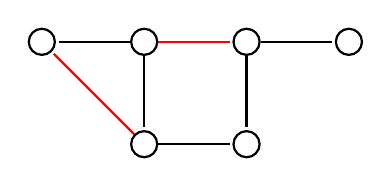
\begin{tikzpicture}[-,>=stealth,shorten >=1pt,auto,node distance=1.3cm, thick,main node/.style={scale=0.9,circle,draw,font=\sffamily\normalsize}]

            \node[circle, draw] (1) []{};
            \node[circle, draw] (2) [right of = 1]{};
            \node[circle, draw] (3) [below of = 1]{};
            \node[circle, draw] (4) [below of = 2]{};
            \node[circle, draw] (5) [left of = 1]{};
            \node[circle, draw] (6) [right of = 2]{};

            \draw[-] (1) [red] to (2);
            \draw[-] (1) to (3);
            \draw[-] (2) to (4);
            \draw[-] (1) to (5);
            \draw[-] (3) to (4);
            \draw[-] (3) [red] to (5);
            \draw[-] (2) to (6);

            ;
        \end{tikzpicture}
        \caption{A \tit{matching} of the previous graph.}
        \label{matching}
    \end{figure}

    As shown in figure, a matching is nothing more than a set of edges that must not share endpoints with each other --- for this reason, in literature it is often referred to as \tbf{independent edge set}. Differently from the vertex cover structure, in this context the trivial matching is clearly the set $A = \varnothing$, which vacuously satisfies the matching condition. However, a more interesting solution is represented by the \tbf{maximum matching}, but this time we have to distinguish two slightly different definitions, namely the concept of \tit{maximal} and \tit{maximum}.

    \begin{frameddefn}{Maximal matching}
        A \tbf{maximal matching} is a matching that cannot be extended any further.
    \end{frameddefn}
    
    For instance, the matching shown in \cref{matching} is actually a \tbf{maximal matching}, because no other edge in $E$ can be added to the current set of edges $A$ of the matching without breaking the matching condition.

    \begin{frameddefn}{Maximum matching}
        A \tbf{maximum matching} is a matching that has the largest cardinality.
    \end{frameddefn}
    
    Clearly, the previous example does not represent a \tbf{maximum matching}, because the following set of edges

    \begin{figure}[H]
        \centering
        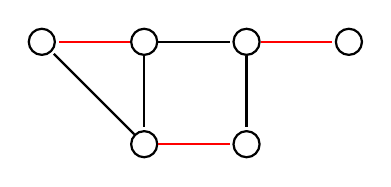
\begin{tikzpicture}[-,>=stealth,shorten >=1pt,auto,node distance=1.3cm, thick,main node/.style={scale=0.9,circle,draw,font=\sffamily\normalsize}]

            \node[circle, draw] (1) []{};
            \node[circle, draw] (2) [right of = 1]{};
            \node[circle, draw] (3) [below of = 1]{};
            \node[circle, draw] (4) [below of = 2]{};
            \node[circle, draw] (5) [left of = 1]{};
            \node[circle, draw] (6) [right of = 2]{};

            \draw[-] (1) to (2);
            \draw[-] (1) to (3);
            \draw[-] (2) to (4);
            \draw[-] (1) [red] to (5);
            \draw[-] (3) [red] to (4);
            \draw[-] (3) to (5);
            \draw[-] (2) [red] to (6);

            ;
        \end{tikzpicture}
    \end{figure}

    is still a valid matching for the graph, but has a larger cardinality than the previous set.

    Differently from the VC problem, a \tit{maximum matching} can be found in polynomial time. Moreover, the following algorithm can be used to determine a \tit{maximal matching} of a given graph.

    \begin{framedalgo}{Maximal matching}
        Given an undirected graph $G = (V, E)$, the algorithm returns a maximal matching of $G$. \\
        \hrule

        \quad
        \begin{algorithmic}[1]
            \Function{MaximalMatching}{$G$}
                \State $S := \varnothing$
                \While{$E \neq \varnothing$}
                    \State Choose $e = \{u, v\} \in E$
                    \State $S = S \cup \{u, v\}$
                    \State Remove from $E$ all the edges incident on $u$ or on $v$
                    \State $E = E - \{e\}$
                \EndWhile
                \State \textbf{return} $S$
            \EndFunction
        \end{algorithmic}
    \end{framedalgo}

    \idea{
        The algorithm is very straightforward: at each iteration, a random edge $e = \{u, v\}$ is chosen from $E$, and then any edge $e' \in E$ such that $e \cap e' \neq \varnothing$ is removed from $E$.

        Clearly, line 6 ensures that the output is a \tit{matching}, and the terminating condition of the \texttt{while} loop ensures that it is \tit{maximal}, but since the output depends on the chosen edges, $S$ is not guaranteed to be \tit{maximum}.
    }

    Additionally, another major reason we focus on matchings is the following theorem.

    \begin{framedthm}{Matchings bound vertex covers}
        Given an undirected graph $G = (V, E)$, a matching $A \subseteq E$ of $G$, and a vertex cover $S \subseteq V$ of $G$, we have that $\abs S \ge \abs A$.
    \end{framedthm}

    \begin{proof}
        By definition, any vertex cover $S$ of $G = (V, E)$ is also a vertex cover for $G^B = (V, B)$, for any set of edges $B \subseteq E$, and in particular this is true for $G^A = (V, A)$.

        Now consider $G^A$, and a vertex cover $C$ on it: by construction we have that $\Delta \le 1$, therefore any vertex in $C$ will cover at most 1 edge of $A$. This implies that if $\abs C = k$, then $C$ will cover at most $k$ edges of $G^A$.

        Lastly, since $G^A$ has $\abs A$ edges by definition, any vertex cover defined on $G^A$ has to contain at least $\abs A$. This implies that no vertex cover $S$ of $G$ smaller than $\abs A$ can exist, because $S$ will have to cover at least the edges in $A$.
    \end{proof}
    
    Thanks to this theorem, we can easily show that the algorithm that we just presented in order to find maximal matchings is a 2-approximation of the VC problem. 

    \begin{framedthm}{2-approximation of VC problem}
        The \textsc{MaximalMatching} algorithm is a 2-approximation of the Vertex Cover problem.
    \end{framedthm}

    \begin{proof}
        Given an undirected $G = (V, E)$, let $S = \textsc{MaximalMatching}(G)$, and let $e_1, \ldots, e_t$ be the sequence of edges chosen by the algorithm at each iteration of the \texttt{while} loop.

        Note that, by definition of the algorithm, at each iteration exactly 2 vertices are added to $S \subseteq V$, and it always holds that $$S_{i + 1} \cap S_i = e_i = \{u, v\}$$ for any iteration $i \in [t - 1]$, because in line 6 the algorithm removes from $E$ all the edges incident on either $u$ or $v$. This implies that $\abs S = 2t$.

        placeholder \todo{the last part is wrong}
    \end{proof}
    
    This 2-approximation algorithm is conjectured to be optimal, but it has not been proven yet. In fact, the VC problem is conjectured to be \NPHard to $(2 - \varepsilon)$-approximate, for any $\varepsilon > 0$.

    Interestingly, the decisional version of the VC problem is \href{https://en.wikipedia.org/wiki/Parameterized_complexity#FPT}{Fixed Parameter Tractable}. This characterization comes from the nature of the problem: for each edge $e = \{u, v\}$ of a given undirected graph $G = (V, E)$, either $u$ or $v$ has to be in the vertex cover, therefore it possible to approach the VC problem by trying all possible choices of set of vertices $S \subseteq V$, and backtrack if necessary. The following algorithm employs this idea.

    \begin{framedalgo}{Decisional VC}
        Given an undirected graph $G = (V, E)$, and an integer $k$, the algorithm returns \texttt{True} if and only if $G$ admits a vertex cover of size $k$. \\
        \hrule

        \quad
        \begin{algorithmic}[1]
            \Function{VC}{$G$, $k$}
                \If{$E == \varnothing$}
                    \State \tbf{return} \texttt{True}
                \ElsIf{$k == 0$}
                    \State \tbf{return} \texttt{False}
                \Else
                    \State Choose $e = \{u, v\} \in E$
                    \If{$\textsc{VC}(G[V - \{u\}]), k - 1)$}
                        \State \tbf{return} \texttt{True}
                    \EndIf
                    \If{$\textsc{VC}(G[V - \{v\}]), k - 1)$}
                        \State \tbf{return} \texttt{True}
                    \EndIf
                    \State \tbf{return} \texttt{False}
                \EndIf
            \EndFunction
        \end{algorithmic}
    \end{framedalgo}

    The algorithm uses the definition of \tbf{induced subgraph}, which is defined as follows.

    \begin{frameddefn}{Induced subgraph}
        Given an undirected graph $G = (V, E)$, and a set of vertices $S \subseteq V$, then $G[S]$ represents the \tbf{subgraph induced by $S$ on $G$}, and it is obtained by removing from $G$ all the nodes of $V - S$ --- and their corresponding edges.
    \end{frameddefn}

     \begin{figure}[H]
        \centering

        \begin{tabular}{ccc}
            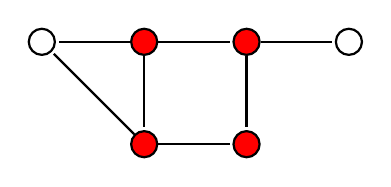
\begin{tikzpicture}[-,>=stealth,shorten >=1pt,auto,node distance=1.3cm, thick,main node/.style={scale=0.9,circle,draw,font=\sffamily\normalsize}]

                \node[circle, draw, fill=red] (1) []{};
                \node[circle, draw, fill=red] (2) [right of = 1]{};
                \node[circle, draw, fill=red] (3) [below of = 1]{};
                \node[circle, draw, fill=red] (4) [below of = 2]{};
                \node[circle, draw] (5) [left of = 1]{};
                \node[circle, draw] (6) [right of = 2]{};

                \draw[-] (1) to (2);
                \draw[-] (1) to (3);
                \draw[-] (2) to (4);
                \draw[-] (1) to (5);
                \draw[-] (3) to (4);
                \draw[-] (3) to (5);
                \draw[-] (2) to (6);

                ;
            \end{tikzpicture}

            &\qquad\qquad&

            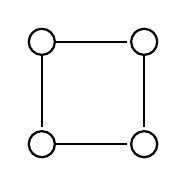
\begin{tikzpicture}[-,>=stealth,shorten >=1pt,auto,node distance=1.3cm, thick,main node/.style={scale=0.9,circle,draw,font=\sffamily\normalsize}]

                \node[circle, draw] (1) []{};
                \node[circle, draw] (2) [right of = 1]{};
                \node[circle, draw] (3) [below of = 1]{};
                \node[circle, draw] (4) [below of = 2]{};

                \draw[-] (1) to (2);
                \draw[-] (1) to (3);
                \draw[-] (2) to (4);
                \draw[-] (3) to (4);

                ;
            \end{tikzpicture}
        \end{tabular}

        \caption{On the left: a graph $G$ and a set of vertices $S$. On the right: the graph $G[S]$.}
    \end{figure}

    \idea{
        The structure of the algorithm consists of a simple backtracking algorithm:
        \begin{itemize}
            \item if the current graph has no edges, we covered every edge of the graph, therefore we return \texttt{True}
            \item if the current graph has some edges, but $k = 0$, then $G$ does not admit a vertex cover of size $k$, thus we return \texttt{False}
            \item if the current graph has some edges, and $k \neq 0$, then we choose an edge $e = \{u, v\} \in E$ arbitrarily, and we try to consider first $u$ then $v$ in a possible vertex cover --- note that $G[V - \{x\}]$ is a graph that does not contain $x$, neither any edge adjacent to it; if both attempts fail, we return \texttt{False}
        \end{itemize}
    }

    \cost{
        It is easy to see that the cost directly depends on the number of recursive calls that the algorithm performs, which is $2^k$ in the worst case, and the cost of constructing $G[V - \{x\}]$, which we can assume to be $O\rbk{n^2}$. Hence, the algorithm has a total cost of $O \rbk{2^k \cdot n^2}$.
    }
   
    \printbibliography % UNCOMMENT FOR BIBLIOGRAPHY

\end{document}
